% Options for packages loaded elsewhere
\PassOptionsToPackage{unicode}{hyperref}
\PassOptionsToPackage{hyphens}{url}
\PassOptionsToPackage{dvipsnames,svgnames,x11names}{xcolor}
%
\documentclass[
  letterpaper,
  DIV=11,
  numbers=noendperiod]{scrartcl}

\usepackage{amsmath,amssymb}
\usepackage{iftex}
\ifPDFTeX
  \usepackage[T1]{fontenc}
  \usepackage[utf8]{inputenc}
  \usepackage{textcomp} % provide euro and other symbols
\else % if luatex or xetex
  \usepackage{unicode-math}
  \defaultfontfeatures{Scale=MatchLowercase}
  \defaultfontfeatures[\rmfamily]{Ligatures=TeX,Scale=1}
\fi
\usepackage{lmodern}
\ifPDFTeX\else  
    % xetex/luatex font selection
\fi
% Use upquote if available, for straight quotes in verbatim environments
\IfFileExists{upquote.sty}{\usepackage{upquote}}{}
\IfFileExists{microtype.sty}{% use microtype if available
  \usepackage[]{microtype}
  \UseMicrotypeSet[protrusion]{basicmath} % disable protrusion for tt fonts
}{}
\makeatletter
\@ifundefined{KOMAClassName}{% if non-KOMA class
  \IfFileExists{parskip.sty}{%
    \usepackage{parskip}
  }{% else
    \setlength{\parindent}{0pt}
    \setlength{\parskip}{6pt plus 2pt minus 1pt}}
}{% if KOMA class
  \KOMAoptions{parskip=half}}
\makeatother
\usepackage{xcolor}
\setlength{\emergencystretch}{3em} % prevent overfull lines
\setcounter{secnumdepth}{5}
% Make \paragraph and \subparagraph free-standing
\ifx\paragraph\undefined\else
  \let\oldparagraph\paragraph
  \renewcommand{\paragraph}[1]{\oldparagraph{#1}\mbox{}}
\fi
\ifx\subparagraph\undefined\else
  \let\oldsubparagraph\subparagraph
  \renewcommand{\subparagraph}[1]{\oldsubparagraph{#1}\mbox{}}
\fi

\usepackage{color}
\usepackage{fancyvrb}
\newcommand{\VerbBar}{|}
\newcommand{\VERB}{\Verb[commandchars=\\\{\}]}
\DefineVerbatimEnvironment{Highlighting}{Verbatim}{commandchars=\\\{\}}
% Add ',fontsize=\small' for more characters per line
\usepackage{framed}
\definecolor{shadecolor}{RGB}{241,243,245}
\newenvironment{Shaded}{\begin{snugshade}}{\end{snugshade}}
\newcommand{\AlertTok}[1]{\textcolor[rgb]{0.68,0.00,0.00}{#1}}
\newcommand{\AnnotationTok}[1]{\textcolor[rgb]{0.37,0.37,0.37}{#1}}
\newcommand{\AttributeTok}[1]{\textcolor[rgb]{0.40,0.45,0.13}{#1}}
\newcommand{\BaseNTok}[1]{\textcolor[rgb]{0.68,0.00,0.00}{#1}}
\newcommand{\BuiltInTok}[1]{\textcolor[rgb]{0.00,0.23,0.31}{#1}}
\newcommand{\CharTok}[1]{\textcolor[rgb]{0.13,0.47,0.30}{#1}}
\newcommand{\CommentTok}[1]{\textcolor[rgb]{0.37,0.37,0.37}{#1}}
\newcommand{\CommentVarTok}[1]{\textcolor[rgb]{0.37,0.37,0.37}{\textit{#1}}}
\newcommand{\ConstantTok}[1]{\textcolor[rgb]{0.56,0.35,0.01}{#1}}
\newcommand{\ControlFlowTok}[1]{\textcolor[rgb]{0.00,0.23,0.31}{#1}}
\newcommand{\DataTypeTok}[1]{\textcolor[rgb]{0.68,0.00,0.00}{#1}}
\newcommand{\DecValTok}[1]{\textcolor[rgb]{0.68,0.00,0.00}{#1}}
\newcommand{\DocumentationTok}[1]{\textcolor[rgb]{0.37,0.37,0.37}{\textit{#1}}}
\newcommand{\ErrorTok}[1]{\textcolor[rgb]{0.68,0.00,0.00}{#1}}
\newcommand{\ExtensionTok}[1]{\textcolor[rgb]{0.00,0.23,0.31}{#1}}
\newcommand{\FloatTok}[1]{\textcolor[rgb]{0.68,0.00,0.00}{#1}}
\newcommand{\FunctionTok}[1]{\textcolor[rgb]{0.28,0.35,0.67}{#1}}
\newcommand{\ImportTok}[1]{\textcolor[rgb]{0.00,0.46,0.62}{#1}}
\newcommand{\InformationTok}[1]{\textcolor[rgb]{0.37,0.37,0.37}{#1}}
\newcommand{\KeywordTok}[1]{\textcolor[rgb]{0.00,0.23,0.31}{#1}}
\newcommand{\NormalTok}[1]{\textcolor[rgb]{0.00,0.23,0.31}{#1}}
\newcommand{\OperatorTok}[1]{\textcolor[rgb]{0.37,0.37,0.37}{#1}}
\newcommand{\OtherTok}[1]{\textcolor[rgb]{0.00,0.23,0.31}{#1}}
\newcommand{\PreprocessorTok}[1]{\textcolor[rgb]{0.68,0.00,0.00}{#1}}
\newcommand{\RegionMarkerTok}[1]{\textcolor[rgb]{0.00,0.23,0.31}{#1}}
\newcommand{\SpecialCharTok}[1]{\textcolor[rgb]{0.37,0.37,0.37}{#1}}
\newcommand{\SpecialStringTok}[1]{\textcolor[rgb]{0.13,0.47,0.30}{#1}}
\newcommand{\StringTok}[1]{\textcolor[rgb]{0.13,0.47,0.30}{#1}}
\newcommand{\VariableTok}[1]{\textcolor[rgb]{0.07,0.07,0.07}{#1}}
\newcommand{\VerbatimStringTok}[1]{\textcolor[rgb]{0.13,0.47,0.30}{#1}}
\newcommand{\WarningTok}[1]{\textcolor[rgb]{0.37,0.37,0.37}{\textit{#1}}}

\providecommand{\tightlist}{%
  \setlength{\itemsep}{0pt}\setlength{\parskip}{0pt}}\usepackage{longtable,booktabs,array}
\usepackage{calc} % for calculating minipage widths
% Correct order of tables after \paragraph or \subparagraph
\usepackage{etoolbox}
\makeatletter
\patchcmd\longtable{\par}{\if@noskipsec\mbox{}\fi\par}{}{}
\makeatother
% Allow footnotes in longtable head/foot
\IfFileExists{footnotehyper.sty}{\usepackage{footnotehyper}}{\usepackage{footnote}}
\makesavenoteenv{longtable}
\usepackage{graphicx}
\makeatletter
\def\maxwidth{\ifdim\Gin@nat@width>\linewidth\linewidth\else\Gin@nat@width\fi}
\def\maxheight{\ifdim\Gin@nat@height>\textheight\textheight\else\Gin@nat@height\fi}
\makeatother
% Scale images if necessary, so that they will not overflow the page
% margins by default, and it is still possible to overwrite the defaults
% using explicit options in \includegraphics[width, height, ...]{}
\setkeys{Gin}{width=\maxwidth,height=\maxheight,keepaspectratio}
% Set default figure placement to htbp
\makeatletter
\def\fps@figure{htbp}
\makeatother
% definitions for citeproc citations
\NewDocumentCommand\citeproctext{}{}
\NewDocumentCommand\citeproc{mm}{%
  \begingroup\def\citeproctext{#2}\cite{#1}\endgroup}
\makeatletter
 % allow citations to break across lines
 \let\@cite@ofmt\@firstofone
 % avoid brackets around text for \cite:
 \def\@biblabel#1{}
 \def\@cite#1#2{{#1\if@tempswa , #2\fi}}
\makeatother
\newlength{\cslhangindent}
\setlength{\cslhangindent}{1.5em}
\newlength{\csllabelwidth}
\setlength{\csllabelwidth}{3em}
\newenvironment{CSLReferences}[2] % #1 hanging-indent, #2 entry-spacing
 {\begin{list}{}{%
  \setlength{\itemindent}{0pt}
  \setlength{\leftmargin}{0pt}
  \setlength{\parsep}{0pt}
  % turn on hanging indent if param 1 is 1
  \ifodd #1
   \setlength{\leftmargin}{\cslhangindent}
   \setlength{\itemindent}{-1\cslhangindent}
  \fi
  % set entry spacing
  \setlength{\itemsep}{#2\baselineskip}}}
 {\end{list}}
\usepackage{calc}
\newcommand{\CSLBlock}[1]{\hfill\break\parbox[t]{\linewidth}{\strut\ignorespaces#1\strut}}
\newcommand{\CSLLeftMargin}[1]{\parbox[t]{\csllabelwidth}{\strut#1\strut}}
\newcommand{\CSLRightInline}[1]{\parbox[t]{\linewidth - \csllabelwidth}{\strut#1\strut}}
\newcommand{\CSLIndent}[1]{\hspace{\cslhangindent}#1}

\usepackage{float}
\usepackage{tabularray}
\usepackage[normalem]{ulem}
\usepackage{graphicx}
\UseTblrLibrary{booktabs}
\UseTblrLibrary{siunitx}
\NewTableCommand{\tinytableDefineColor}[3]{\definecolor{#1}{#2}{#3}}
\newcommand{\tinytableTabularrayUnderline}[1]{\underline{#1}}
\newcommand{\tinytableTabularrayStrikeout}[1]{\sout{#1}}
\KOMAoption{captions}{tableheading}
\makeatletter
\@ifpackageloaded{caption}{}{\usepackage{caption}}
\AtBeginDocument{%
\ifdefined\contentsname
  \renewcommand*\contentsname{Table of contents}
\else
  \newcommand\contentsname{Table of contents}
\fi
\ifdefined\listfigurename
  \renewcommand*\listfigurename{List of Figures}
\else
  \newcommand\listfigurename{List of Figures}
\fi
\ifdefined\listtablename
  \renewcommand*\listtablename{List of Tables}
\else
  \newcommand\listtablename{List of Tables}
\fi
\ifdefined\figurename
  \renewcommand*\figurename{Figure}
\else
  \newcommand\figurename{Figure}
\fi
\ifdefined\tablename
  \renewcommand*\tablename{Table}
\else
  \newcommand\tablename{Table}
\fi
}
\@ifpackageloaded{float}{}{\usepackage{float}}
\floatstyle{ruled}
\@ifundefined{c@chapter}{\newfloat{codelisting}{h}{lop}}{\newfloat{codelisting}{h}{lop}[chapter]}
\floatname{codelisting}{Listing}
\newcommand*\listoflistings{\listof{codelisting}{List of Listings}}
\makeatother
\makeatletter
\makeatother
\makeatletter
\@ifpackageloaded{caption}{}{\usepackage{caption}}
\@ifpackageloaded{subcaption}{}{\usepackage{subcaption}}
\makeatother
\ifLuaTeX
  \usepackage{selnolig}  % disable illegal ligatures
\fi
\usepackage{bookmark}

\IfFileExists{xurl.sty}{\usepackage{xurl}}{} % add URL line breaks if available
\urlstyle{same} % disable monospaced font for URLs
\hypersetup{
  pdftitle={Is it time for an NBA expansion?},
  pdfauthor={Yan Mezhiborsky},
  colorlinks=true,
  linkcolor={blue},
  filecolor={Maroon},
  citecolor={Blue},
  urlcolor={Blue},
  pdfcreator={LaTeX via pandoc}}

\title{Is it time for an NBA expansion?\thanks{Code and data are
available at: https://github.com/Mezhi18/NBAExpansion .}}
\usepackage{etoolbox}
\makeatletter
\providecommand{\subtitle}[1]{% add subtitle to \maketitle
  \apptocmd{\@title}{\par {\large #1 \par}}{}{}
}
\makeatother
\subtitle{My subtitle if needed}
\author{Yan Mezhiborsky}
\date{April 14, 2024}

\begin{document}
\maketitle
\begin{abstract}
First sentence. Second sentence. Third sentence. Fourth sentence.
\end{abstract}

\renewcommand*\contentsname{Table of contents}
{
\hypersetup{linkcolor=}
\setcounter{tocdepth}{3}
\tableofcontents
}
\section{Introduction}\label{introduction}

You can and should cross-reference sections and sub-sections. We use R
Core Team (2023) and Wickham et al. (2019).

The remainder of this paper is structured as follows.
Section~\ref{sec-data}\ldots.

\section{Data}\label{sec-data}

Some of our data is of penguins (\textbf{?@fig-bills}), from Horst,
Hill, and Gorman (2020).

Talk more about it.

And also planes (\textbf{?@fig-planes}). (You can change the height and
width, but don't worry about doing that until you have finished every
other aspect of the paper - Quarto will try to make it look nice and the
defaults usually work well once you have enough text.)

Talk way more about it.

\section{Model}\label{model}

The goal of our modelling strategy is twofold. Firstly,\ldots{}

Here we briefly describe the Bayesian analysis model used to
investigate\ldots{} Background details and diagnostics are included in
Appendix~\ref{sec-model-details}.

\subsection{Model set-up}\label{model-set-up}

Define \(y_i\) as the average number of points per game scored by a team
through out the NBA season. Then \(\alpha\) is the average assists per
game, \(\rho\) the average rebounds per game, \(\beta\) is blocks per
game, \(\psi\) is steals per game and lastly, \(\tau\) is turnovers per
game.

\begin{align} 
y_i|\mu_i, \sigma &\sim \mbox{Normal}(\mu_i, \sigma) \\
\mu_i &= \alpha + \rho_i + \beta_i + \xi_i + \tau_i \\
\alpha &\sim \mbox{Normal}(0, 2.5) \\
\rho &\sim \mbox{Normal}(0, 2.5) \\
\beta &\sim \mbox{Normal}(0, 2.5) \\
\psi &\sim \mbox{Normal}(0,2.5) \\
\tau &\sim \mbox{Normal}(0,2.5) \\
\sigma &\sim \mbox{Exponential}(1) \\
\end{align}

\begin{Shaded}
\begin{Highlighting}[]
\CommentTok{\# Simulating data}
\FunctionTok{set.seed}\NormalTok{(}\DecValTok{123}\NormalTok{)  }\CommentTok{\# For reproducibility}
\NormalTok{sim\_nba\_data }\OtherTok{\textless{}{-}} \FunctionTok{data.frame}\NormalTok{(}
  \AttributeTok{Year =} \FunctionTok{rep}\NormalTok{(}\DecValTok{1980}\SpecialCharTok{:}\DecValTok{2023}\NormalTok{, }\AttributeTok{times =} \DecValTok{10}\NormalTok{),  }\CommentTok{\# Simulate 10 records per year}
  \AttributeTok{Num\_teams =} \FunctionTok{c}\NormalTok{(}\FunctionTok{rep}\NormalTok{(}\DecValTok{22}\NormalTok{, }\AttributeTok{each =} \DecValTok{1} \SpecialCharTok{*} \DecValTok{10}\NormalTok{),}
                \FunctionTok{rep}\NormalTok{(}\DecValTok{23}\NormalTok{, }\AttributeTok{each =} \DecValTok{8} \SpecialCharTok{*} \DecValTok{10}\NormalTok{),}
                \FunctionTok{rep}\NormalTok{(}\DecValTok{25}\NormalTok{, }\AttributeTok{each =} \DecValTok{1} \SpecialCharTok{*} \DecValTok{10}\NormalTok{),}
                \FunctionTok{rep}\NormalTok{(}\DecValTok{27}\NormalTok{, }\AttributeTok{each =} \DecValTok{6} \SpecialCharTok{*} \DecValTok{10}\NormalTok{),}
                \FunctionTok{rep}\NormalTok{(}\DecValTok{29}\NormalTok{, }\AttributeTok{each =} \DecValTok{9} \SpecialCharTok{*} \DecValTok{10}\NormalTok{),}
                \FunctionTok{rep}\NormalTok{(}\DecValTok{30}\NormalTok{, }\AttributeTok{each =} \DecValTok{19} \SpecialCharTok{*} \DecValTok{10}\NormalTok{)),  }\CommentTok{\# Adjusted each parameter as needed}
  \AttributeTok{PTS =} \FunctionTok{rnorm}\NormalTok{(}\DecValTok{440}\NormalTok{, }\AttributeTok{mean =} \FunctionTok{mean}\NormalTok{(full\_nba\_data}\SpecialCharTok{$}\NormalTok{PTS), }\AttributeTok{sd =} \FunctionTok{sd}\NormalTok{(full\_nba\_data}\SpecialCharTok{$}\NormalTok{PTS)),  }
  \AttributeTok{AST =} \FunctionTok{rnorm}\NormalTok{(}\DecValTok{440}\NormalTok{, }\AttributeTok{mean =} \FunctionTok{mean}\NormalTok{(full\_nba\_data}\SpecialCharTok{$}\NormalTok{AST), }\AttributeTok{sd =} \FunctionTok{sd}\NormalTok{(full\_nba\_data}\SpecialCharTok{$}\NormalTok{AST)), }
  \AttributeTok{TRB =} \FunctionTok{rnorm}\NormalTok{(}\DecValTok{440}\NormalTok{, }\AttributeTok{mean =} \FunctionTok{mean}\NormalTok{(full\_nba\_data}\SpecialCharTok{$}\NormalTok{TRB), }\AttributeTok{sd =} \FunctionTok{sd}\NormalTok{(full\_nba\_data}\SpecialCharTok{$}\NormalTok{TRB)),  }
  \AttributeTok{STL =} \FunctionTok{rnorm}\NormalTok{(}\DecValTok{440}\NormalTok{, }\AttributeTok{mean =} \FunctionTok{mean}\NormalTok{(full\_nba\_data}\SpecialCharTok{$}\NormalTok{STL), }\AttributeTok{sd =} \FunctionTok{sd}\NormalTok{(full\_nba\_data}\SpecialCharTok{$}\NormalTok{STL)),  }
  \AttributeTok{BLK =} \FunctionTok{rnorm}\NormalTok{(}\DecValTok{440}\NormalTok{, }\AttributeTok{mean =} \FunctionTok{mean}\NormalTok{(full\_nba\_data}\SpecialCharTok{$}\NormalTok{BLK), }\AttributeTok{sd =} \FunctionTok{sd}\NormalTok{(full\_nba\_data}\SpecialCharTok{$}\NormalTok{BLK)),  }
  \AttributeTok{TOV =} \FunctionTok{rnorm}\NormalTok{(}\DecValTok{440}\NormalTok{, }\AttributeTok{mean =} \FunctionTok{mean}\NormalTok{(full\_nba\_data}\SpecialCharTok{$}\NormalTok{TOV), }\AttributeTok{sd =} \FunctionTok{sd}\NormalTok{(full\_nba\_data}\SpecialCharTok{$}\NormalTok{TOV)) }
\NormalTok{)}
\CommentTok{\# Add a column for PPG that depends on the year and number of teams, }
\CommentTok{\# as well as other factors. Adjust the coefficients as needed for your simulation.}
\NormalTok{sim\_nba\_data\_1 }\OtherTok{\textless{}{-}}\NormalTok{ sim\_nba\_data }\SpecialCharTok{\%\textgreater{}\%}
  \FunctionTok{mutate}\NormalTok{(}\AttributeTok{PPG =}\NormalTok{ (PTS }\SpecialCharTok{/} \DecValTok{82}\NormalTok{) }\SpecialCharTok{+}\NormalTok{ (Year }\SpecialCharTok{{-}} \DecValTok{1980}\NormalTok{) }\SpecialCharTok{*} \FloatTok{0.2} \SpecialCharTok{{-}}\NormalTok{ (Num\_teams }\SpecialCharTok{{-}} \DecValTok{22}\NormalTok{) }\SpecialCharTok{*} \FloatTok{0.1} \SpecialCharTok{+}
                \FloatTok{0.1} \SpecialCharTok{*}\NormalTok{ AST }\SpecialCharTok{+} \FloatTok{0.05} \SpecialCharTok{*}\NormalTok{ TRB }\SpecialCharTok{{-}} \FloatTok{0.05} \SpecialCharTok{*}\NormalTok{ STL }\SpecialCharTok{+} \FloatTok{0.05} \SpecialCharTok{*}\NormalTok{ BLK }\SpecialCharTok{{-}} \FloatTok{0.05} \SpecialCharTok{*}\NormalTok{ TOV)}

\CommentTok{\# Fit a multiple linear regression model}
\NormalTok{nba\_model }\OtherTok{\textless{}{-}} \FunctionTok{lm}\NormalTok{(PTS }\SpecialCharTok{\textasciitilde{}}\NormalTok{ Year }\SpecialCharTok{*}\NormalTok{ Num\_teams }\SpecialCharTok{+}\NormalTok{ AST }\SpecialCharTok{+}\NormalTok{ TRB }\SpecialCharTok{+}\NormalTok{ STL }\SpecialCharTok{+}\NormalTok{ BLK }\SpecialCharTok{+}\NormalTok{ TOV, }\AttributeTok{data =}\NormalTok{ sim\_nba\_data)}
\NormalTok{nba\_model\_1 }\OtherTok{\textless{}{-}} \FunctionTok{lm}\NormalTok{(PTS }\SpecialCharTok{\textasciitilde{}}\NormalTok{ Year }\SpecialCharTok{*}\NormalTok{ Num\_teams }\SpecialCharTok{+}\NormalTok{ AST }\SpecialCharTok{+}\NormalTok{ TRB }\SpecialCharTok{+}\NormalTok{ STL }\SpecialCharTok{+}\NormalTok{ BLK }\SpecialCharTok{+}\NormalTok{ TOV, }\AttributeTok{data =}\NormalTok{ sim\_nba\_data\_1)}

\CommentTok{\# Summary of the linear model}
\FunctionTok{msummary}\NormalTok{(nba\_model)}
\end{Highlighting}
\end{Shaded}

\begin{table}
\centering
\begin{tblr}[         %% tabularray outer open
]                     %% tabularray outer close
{                     %% tabularray inner open
colspec={Q[]Q[]},
column{1}={halign=l,},
column{2}={halign=c,},
hline{20}={1,2}{solid, 0.05em, black},
}                     %% tabularray inner close
\toprule
& (1) \\ \midrule %% TinyTableHeader
(Intercept)        & \num{-49.339}   \\
& (\num{535.291}) \\
Year               & \num{0.085}     \\
& (\num{0.268})   \\
Num\_teams        & \num{7.500}     \\
& (\num{19.164})  \\
AST                & \num{-0.154}    \\
& (\num{0.132})   \\
TRB                & \num{-0.327}    \\
& (\num{0.166})   \\
STL                & \num{0.153}     \\
& (\num{0.320})   \\
BLK                & \num{-0.417}    \\
& (\num{0.385})   \\
TOV                & \num{0.073}     \\
& (\num{0.193})   \\
Year × Num\_teams & \num{-0.004}    \\
& (\num{0.010})   \\
Num.Obs.           & \num{440}       \\
R2                 & \num{0.017}     \\
R2 Adj.            & \num{-0.001}    \\
AIC                & \num{2997.1}    \\
BIC                & \num{3038.0}    \\
Log.Lik.           & \num{-1488.559} \\
RMSE               & \num{7.13}      \\
\bottomrule
\end{tblr}
\end{table}

\begin{Shaded}
\begin{Highlighting}[]
\FunctionTok{modelsummary}\NormalTok{(nba\_model\_1)}
\end{Highlighting}
\end{Shaded}

\begin{table}
\centering
\begin{tblr}[         %% tabularray outer open
]                     %% tabularray outer close
{                     %% tabularray inner open
colspec={Q[]Q[]},
column{1}={halign=l,},
column{2}={halign=c,},
hline{20}={1,2}{solid, 0.05em, black},
}                     %% tabularray inner close
\toprule
& (1) \\ \midrule %% TinyTableHeader
(Intercept)        & \num{-49.339}   \\
& (\num{535.291}) \\
Year               & \num{0.085}     \\
& (\num{0.268})   \\
Num\_teams        & \num{7.500}     \\
& (\num{19.164})  \\
AST                & \num{-0.154}    \\
& (\num{0.132})   \\
TRB                & \num{-0.327}    \\
& (\num{0.166})   \\
STL                & \num{0.153}     \\
& (\num{0.320})   \\
BLK                & \num{-0.417}    \\
& (\num{0.385})   \\
TOV                & \num{0.073}     \\
& (\num{0.193})   \\
Year × Num\_teams & \num{-0.004}    \\
& (\num{0.010})   \\
Num.Obs.           & \num{440}       \\
R2                 & \num{0.017}     \\
R2 Adj.            & \num{-0.001}    \\
AIC                & \num{2997.1}    \\
BIC                & \num{3038.0}    \\
Log.Lik.           & \num{-1488.559} \\
RMSE               & \num{7.13}      \\
\bottomrule
\end{tblr}
\end{table}

We run the model in R (R Core Team 2023) using the \texttt{rstanarm}
package of Goodrich et al. (2022). We use the default priors from
\texttt{rstanarm}.

\subsubsection{Model justification}\label{model-justification}

We expect a positive relationship between the size of the wings and time
spent aloft. In particular\ldots{}

We can use maths by including latex between dollar signs, for instance
\(\theta\).

\section{Results}\label{results}

Our results are summarized in \textbf{?@tbl-modelresults}.

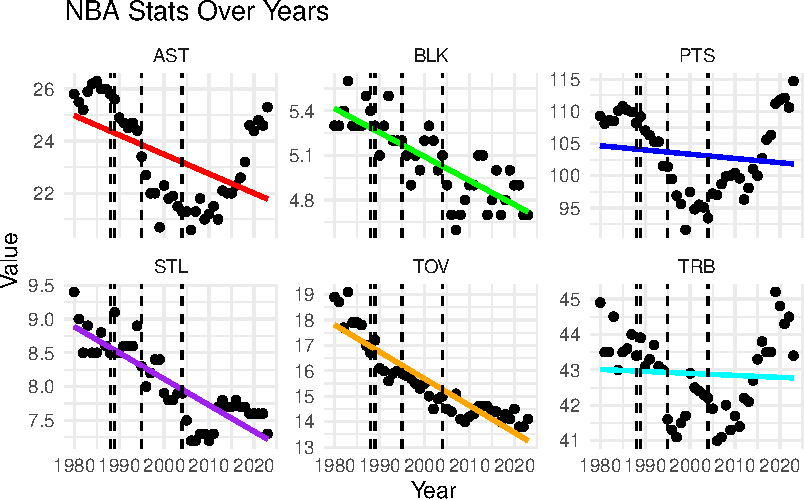
\includegraphics{paper_files/figure-pdf/unnamed-chunk-6-1.pdf}

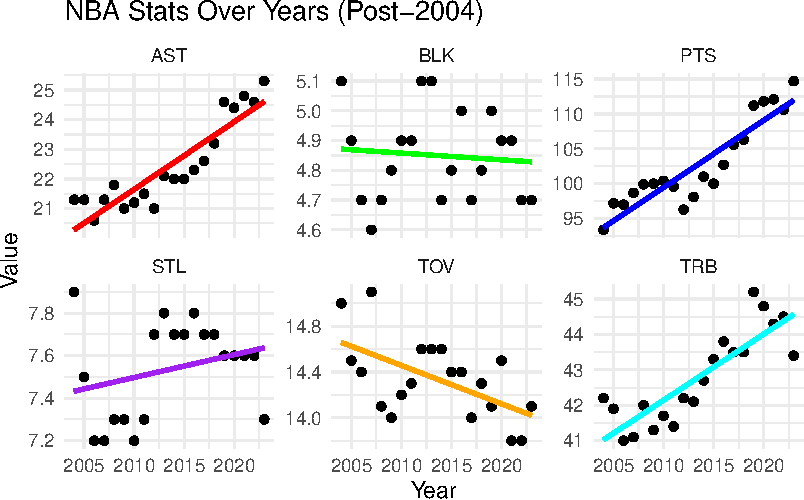
\includegraphics{paper_files/figure-pdf/unnamed-chunk-7-1.pdf}

\section{Discussion}\label{discussion}

\subsection{First discussion point}\label{sec-first-point}

If my paper were 10 pages, then should be be at least 2.5 pages. The
discussion is a chance to show off what you know and what you learnt
from all this.

\subsection{Second discussion point}\label{second-discussion-point}

\subsection{Third discussion point}\label{third-discussion-point}

\subsection{Weaknesses and next steps}\label{weaknesses-and-next-steps}

Weaknesses and next steps should also be included.

\newpage

\appendix

\section*{Appendix}\label{appendix}
\addcontentsline{toc}{section}{Appendix}

\section{Additional data details}\label{additional-data-details}

\section{Model details}\label{sec-model-details}

\subsection{Posterior predictive
check}\label{posterior-predictive-check}

In \textbf{?@fig-ppcheckandposteriorvsprior-1} we implement a posterior
predictive check. This shows\ldots{}

In \textbf{?@fig-ppcheckandposteriorvsprior-2} we compare the posterior
with the prior. This shows\ldots{}

\subsection{Diagnostics}\label{diagnostics}

\textbf{?@fig-stanareyouokay-1} is a trace plot. It shows\ldots{} This
suggests\ldots{}

\textbf{?@fig-stanareyouokay-2} is a Rhat plot. It shows\ldots{} This
suggests\ldots{}

\newpage

\section*{References}\label{references}
\addcontentsline{toc}{section}{References}

\phantomsection\label{refs}
\begin{CSLReferences}{1}{0}
\bibitem[\citeproctext]{ref-rstanarm}
Goodrich, Ben, Jonah Gabry, Imad Ali, and Sam Brilleman. 2022.
{``Rstanarm: {Bayesian} Applied Regression Modeling via {Stan}.''}
\url{https://mc-stan.org/rstanarm/}.

\bibitem[\citeproctext]{ref-palmerpenguins}
Horst, Allison Marie, Alison Presmanes Hill, and Kristen B Gorman. 2020.
\emph{Palmerpenguins: Palmer Archipelago (Antarctica) Penguin Data}.
\url{https://doi.org/10.5281/zenodo.3960218}.

\bibitem[\citeproctext]{ref-citeR}
R Core Team. 2023. \emph{R: A Language and Environment for Statistical
Computing}. Vienna, Austria: R Foundation for Statistical Computing.
\url{https://www.R-project.org/}.

\bibitem[\citeproctext]{ref-rohan}
Wickham, Hadley, Mara Averick, Jennifer Bryan, Winston Chang, Lucy
D'Agostino McGowan, Romain François, Garrett Grolemund, et al. 2019.
{``Welcome to the {tidyverse}.''} \emph{Journal of Open Source Software}
4 (43): 1686. \url{https://doi.org/10.21105/joss.01686}.

\end{CSLReferences}



\end{document}
